\documentclass[border=1pt]{standalone}
% Shared preamble for standalone figures in this directory.
% Compile with XeLaTeX from 讲义/figs, or via the figures target.
\usepackage{ctex}
\usepackage{amsmath}
\usepackage{amssymb}
\usepackage{bm}
\usepackage{mathtools}
\usepackage{tikz}
\renewcommand{\vec}[1]{\boldsymbol{#1}}
\newcommand{\cC}{\mathcal{C}}
\newcommand{\cD}{\mathcal{D}}
\newcommand{\R}{\mathbf{R}}
\usetikzlibrary{
    arrows.meta,
    calc,
    decorations.markings,
    angles,
    quotes,
    positioning,
    patterns,
    shapes.geometric
}

\begin{document}
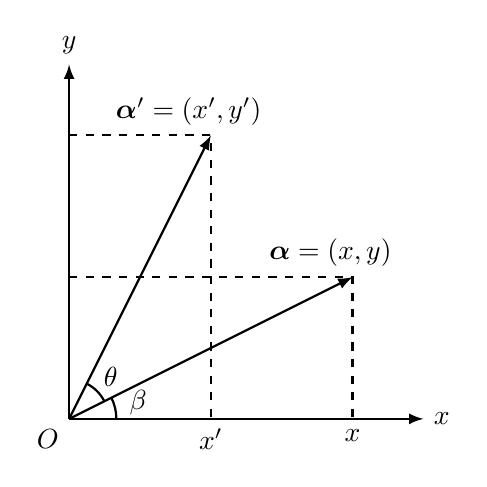
\begin{tikzpicture}[scale=1.8]
    \tikzset{>=latex, every path/.style={thick}}
    \draw (0,0) coordinate (O)
        (1,2) coordinate (A)
        (2,1) coordinate (B)
        (2,0) coordinate (C);
    \draw[->] (0, 0) -- (0, 2.5)
        node[above] {$y$};
    \draw[->] (0, 0) -- (2.5, 0)
        node[right] {$x$};
    \draw[->] (O) -- (A)
        node[above,xshift=-8pt] {$\boldsymbol{\alpha}'=(x',y')$};
    \draw[->] (O) -- (B)
        node[above,xshift=-8pt] {$\boldsymbol{\alpha}=(x,y)$};
    \draw[dashed] (0,2) -- (1,2) -- (1,0) node[below] {$x'$}
        (0,1) -- (2,1) -- (2,0) node[below] {$x$};
    \draw pic[draw,"$\theta$",angle eccentricity=1.5] {angle=B--O--A};
    \draw pic[draw,"$\beta$",angle eccentricity=1.5,angle radius=.6cm] {angle=C--O--B};
    \draw node[below left] at (O) {$O$};
\end{tikzpicture}

\end{document}
